% Uncertainty Response Comparison
% TikZ diagram for Chapter 5 - Fixed vs. Adaptive SMC under parameter variations

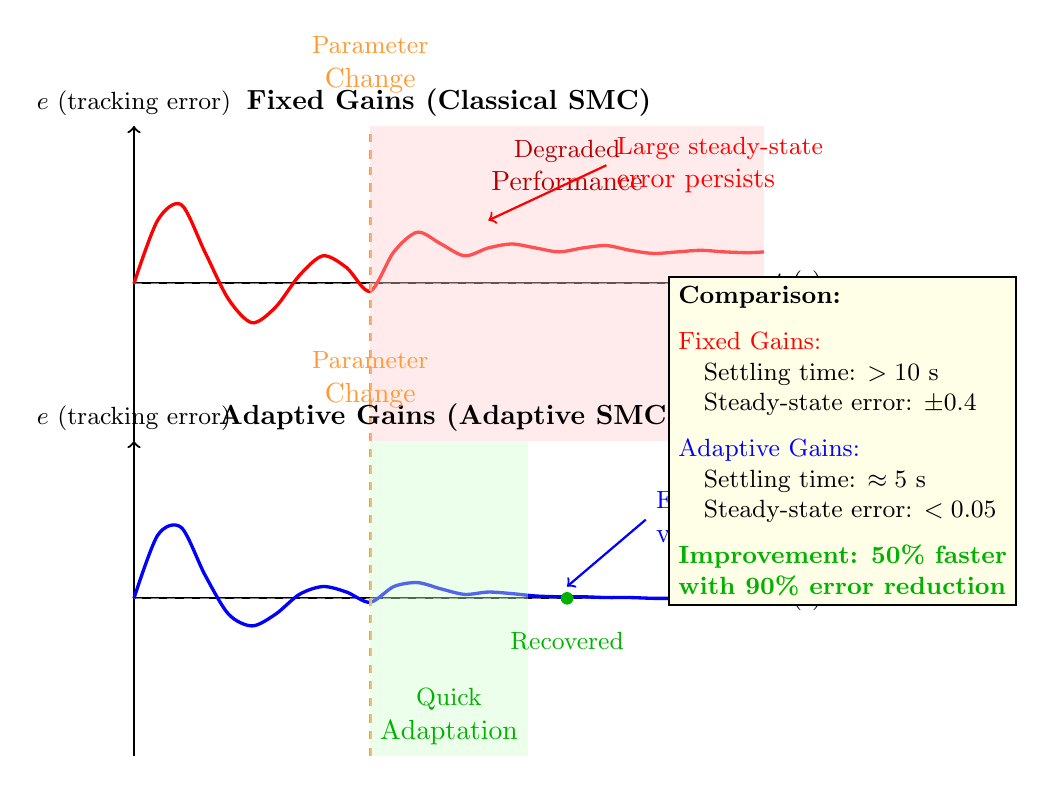
\begin{tikzpicture}[scale=1.0]

    % Fixed SMC subplot (top)
    \begin{scope}[yshift=4cm]
        % Axes
        \draw[->, thick] (0, 0) -- (8, 0) node[right] {\small $t$ (s)};
        \draw[->, thick] (0, -2) -- (0, 2) node[above] {\small $e$ (tracking error)};

        % Title
        \node[above] at (4, 2) {\textbf{Fixed Gains (Classical SMC)}};

        % Reference (zero line)
        \draw[dashed, gray] (0, 0) -- (8, 0);

        % Tracking error with poor response to uncertainty - using coordinates
        \draw[red, very thick, smooth] plot coordinates {
            (0,0) (0.3,0.8) (0.6,1.0) (0.9,0.4) (1.2,-0.2) (1.5,-0.5) (1.8,-0.3)
            (2.1,0.1) (2.4,0.35) (2.7,0.2) (3.0,-0.1) (3.3,0.4) (3.6,0.65)
            (3.9,0.5) (4.2,0.35) (4.5,0.45) (4.8,0.5) (5.1,0.45) (5.4,0.4)
            (5.7,0.45) (6.0,0.48) (6.3,0.42) (6.6,0.38) (6.9,0.4) (7.2,0.42)
            (7.5,0.4) (7.8,0.39) (8.0,0.4)
        };

        % Parameter change marker
        \draw[orange!80, very thick, dashed] (3, -2) -- (3, 2);
        \node[orange!80, above, align=center] at (3, 2.3) {\small Parameter\\Change};

        % Performance degradation region
        \fill[red!20, opacity=0.4] (3, -2) rectangle (8, 2);
        \node[red!70!black, align=center] at (5.5, 1.5) {\small Degraded\\Performance};

        % Annotation
        \draw[<-, thick, red] (4.5, 0.8) -- (6, 1.5)
            node[right, align=left] {\small Large steady-state\\error persists};
    \end{scope}

    % Adaptive SMC subplot (bottom)
    \begin{scope}
        % Axes
        \draw[->, thick] (0, 0) -- (8, 0) node[right] {\small $t$ (s)};
        \draw[->, thick] (0, -2) -- (0, 2) node[above] {\small $e$ (tracking error)};

        % Title
        \node[above] at (4, 2) {\textbf{Adaptive Gains (Adaptive SMC)}};

        % Reference (zero line)
        \draw[dashed, gray] (0, 0) -- (8, 0);

        % Tracking error with good adaptation - using coordinates
        \draw[blue, very thick, smooth] plot coordinates {
            (0,0) (0.3,0.8) (0.6,0.9) (0.9,0.3) (1.2,-0.2) (1.5,-0.35) (1.8,-0.2)
            (2.1,0.05) (2.4,0.15) (2.7,0.08) (3.0,-0.05) (3.3,0.15) (3.6,0.2)
            (3.9,0.12) (4.2,0.05) (4.5,0.08) (4.8,0.06) (5.1,0.03) (5.4,0.02)
            (5.7,0.02) (6.0,0.01) (6.3,0.01) (6.6,0.0) (6.9,0.0) (7.2,0.0)
            (7.5,0.0) (7.8,0.0) (8.0,0.0)
        };

        % Parameter change marker
        \draw[orange!80, very thick, dashed] (3, -2) -- (3, 2);
        \node[orange!80, above, align=center] at (3, 2.3) {\small Parameter\\Change};

        % Adaptation response region
        \fill[green!20, opacity=0.4] (3, -2) rectangle (5, 2);
        \node[green!70!black, align=center] at (4, -1.5) {\small Quick\\Adaptation};

        % Annotation
        \draw[<-, thick, blue] (5.5, 0.15) -- (6.5, 1)
            node[right, align=left] {\small Error reduced\\via gain adaptation};

        % Convergence marker
        \fill[green!70!black] (5.5, 0) circle (0.08);
        \node[green!70!black, below] at (5.5, -0.3) {\small Recovered};
    \end{scope}

    % Comparison metrics
    \begin{scope}[xshift=9cm, yshift=2cm]
        \node[draw, thick, fill=yellow!10, align=left, font=\small] at (0, 0) {
            \textbf{Comparison:}\\[0.2cm]
            \textcolor{red}{Fixed Gains:}\\
            \quad Settling time: $>10$ s\\
            \quad Steady-state error: $\pm0.4$\\[0.2cm]
            \textcolor{blue}{Adaptive Gains:}\\
            \quad Settling time: $\approx 5$ s\\
            \quad Steady-state error: $<0.05$\\[0.2cm]
            \textcolor{green!70!black}{\textbf{Improvement: 50\% faster}}\\
            \textcolor{green!70!black}{\textbf{with 90\% error reduction}}
        };
    \end{scope}

\end{tikzpicture}
